\documentclass[11pt,a4paper,parskip=half]{scrartcl}

\usepackage[T1]{fontenc}
\usepackage{lmodern}
\usepackage[ngerman]{babel}
\usepackage{microtype}
\usepackage[a4paper,top=24mm,bottom=24mm,left=25mm,right=25mm]{geometry}
\usepackage{graphicx}
\usepackage{booktabs}
\usepackage{tabularx}
\usepackage{longtable}
\usepackage{array}
\usepackage{xcolor}
\usepackage{tikz}
\usetikzlibrary{arrows.meta,positioning}
\usepackage{enumitem}
\usepackage{listings}
\usepackage{url}
\usepackage[hidelinks]{hyperref}
\usepackage[nameinlink,noabbrev]{cleveref}
\crefname{section}{Abschnitt}{Abschnitte}
\Crefname{section}{Abschnitt}{Abschnitte}
\crefname{figure}{Abbildung}{Abbildungen}
\Crefname{figure}{Abbildung}{Abbildungen}
\crefname{table}{Tabelle}{Tabellen}
\Crefname{table}{Tabelle}{Tabellen}

\addtokomafont{section}{\sffamily\color{blue!35!black}}
\addtokomafont{subsection}{\sffamily\color{blue!35!black}}
\addtokomafont{subsubsection}{\sffamily\color{blue!35!black}}
\setkomafont{caption}{\small}
\setkomafont{captionlabel}{\bfseries}
\setlist{nosep,leftmargin=1.6em}
\renewcommand{\arraystretch}{1.15}
\graphicspath{{../../experiments/figures/final/}}

\definecolor{projectblue}{HTML}{1F334D}
\definecolor{projectyellow}{HTML}{F2C94C}
\definecolor{importred}{HTML}{C44545}
\definecolor{exportblue}{HTML}{326DB6}
\definecolor{renewgreen}{HTML}{63A35C}

\lstset{
  basicstyle=\ttfamily\small,
  frame=single,
  rulecolor=\color{black!20},
  backgroundcolor=\color{black!2},
  breaklines=true,
  columns=fullflexible,
  keepspaces=true,
  showstringspaces=false
}

\newcommand{\code}[1]{\texttt{#1}}
\newcommand{\gw}{\,GW}
\newcommand{\mwh}{\,EUR/MWh}
\newcommand{\projectlink}[1]{\href{https://gitlab-lehre.informatik.uni-halle.de/aquhr/energiechart-visualisierungsprojekt}{#1}}

\title{Deutschlands Rolle im europäischen Stromnetz\\[0.4em]
  \large Eine interaktive Visual-Analytics-Anwendung mit Elm}
\author{Jann Körner}
\date{21. September 2026}

\begin{document}

\begin{titlepage}
  \centering
  {\sffamily\large Projektbericht zum Modul Informationsvisualisierung\par}
  \vspace{0.3cm}
  {\sffamily\large Sommersemester 2026\par}
  \vfill
  {\sffamily\bfseries\color{projectblue}\fontsize{25}{31}\selectfont
    Deutschlands Rolle im europäischen Stromnetz\par}
  \vspace{0.8cm}
  {\sffamily\Large Eine interaktive Visual-Analytics-Anwendung mit Elm\par}
  \vfill
  {\large Jann Körner\par}
  \vspace{0.35cm}
  {\large 21. September 2026\par}
  \vspace{1.2cm}
  \begin{tikzpicture}
    \fill[projectblue] (0,0) rectangle (11.6,0.20);
    \fill[projectyellow] (0,0.25) rectangle (4.2,0.45);
    \fill[exportblue] (4.3,0.25) rectangle (8.0,0.45);
    \fill[importred] (8.1,0.25) rectangle (11.6,0.45);
  \end{tikzpicture}
  \vfill
  {\small \projectlink{Quellcode und Anwendung im Hochschul-GitLab}\par}
\end{titlepage}

\pagenumbering{roman}
\tableofcontents
\clearpage
\listoffigures
\clearpage
\pagenumbering{arabic}

\section{Einleitung}
\label{sec:einleitung}

Deutschland ist nicht als isoliertes Stromsystem zu verstehen. Erzeugung,
Verbrauch und Handel sind in einen europäischen Verbund eingebettet, während
die tatsächlich gemessenen physikalischen Flüsse den elektrotechnischen
Eigenschaften des Netzes folgen. Handelsmenge und physischer Grenzfluss können
deshalb für dasselbe Länderpaar voneinander abweichen. Gleichzeitig verändern
sich erneuerbare Erzeugung und Day-Ahead-Preis stündlich. Wer Deutschlands Rolle
als Importeur oder Exporteur untersuchen möchte, muss daher räumliche,
zeitliche und mehrdimensionale Zusammenhänge gemeinsam betrachten.

Das Zielproblem dieses Projekts ist die explorative Analyse dieser
Zusammenhänge in einer einzigen Webanwendung. Eine blo{\ss}e Tabelle beantwortet
zwar einzelne Wertfragen, erschwert aber das Erkennen von Zeitmustern,
Richtungswechseln und länderübergreifenden Unterschieden. Umgekehrt würde eine
einzige aggregierte Kurve die Struktur der Partnerländer verdecken. Daraus
ergibt sich die Forschungsfrage:

\begin{quote}
\itshape
Wann ist Deutschland im betrachteten Zeitraum Stromimporteur oder
Stromexporteur, mit welchen Ländern findet der physische Austausch statt und
wie hängen diese Flüsse zeitlich mit Erzeugungsmix und Day-Ahead-Preis zusammen?
\end{quote}

Die Formulierung ist bewusst explorativ. Die Anwendung soll Muster sichtbar
machen und konkrete Stunden vergleichbar machen; sie soll keine Kausalmodelle,
Netzlastflussrechnung oder Herkunftsnachweise für einzelne Strommengen
ersetzen. Insbesondere bedeutet zeitliche Gleichläufigkeit nicht, dass eine
Erzeugungsart einen bestimmten Grenzfluss verursacht.

Das Vorgehen orientiert sich am verschachtelten Prozessmodell von Munzner:
Zuerst werden Anwendungssituation und Aufgaben beschrieben, danach folgen
Daten- und Aufgabenabstraktion, visuelle Kodierung und schlie{\ss}lich die
algorithmische Umsetzung \cite{munzner2009nested}. So wird vermieden, zuerst
leicht implementierbare Diagramme auszuwählen und die Fragestellung im
Nachhinein an diese anzupassen.

\subsection{Anwendungshintergrund}
\label{sec:hintergrund}

Im europäischen Verbundnetz verbinden Grenzkuppelleitungen benachbarte
Gebotszonen. Ein physischer Fluss beschreibt den gemessenen realen
Leistungsaustausch über eine solche Grenze. Ein Handelsfluss ist dagegen ein
kommerzielles Ergebnis gekoppelter Märkte. Physischer und kommerzieller Fluss
stimmen im Allgemeinen nicht überein, weil elektrische Leistung nicht dem
vertraglich gedachten kürzesten Weg folgt, sondern sich entsprechend der
Netzimpedanzen auf Leitungen verteilt \cite{smardFlows}. Die Anwendung stellt
beide Grö{\ss}en deshalb nicht gleich: Physische Flüsse bestimmen die grafische
Richtung und Stärke, Handelswerte werden als zusätzlicher Detailwert im
Tooltip gezeigt.

Die betrachtete deutsche Erzeugung ist ein Leistungsmix aus erneuerbaren und
konventionellen Technologien. Solar- und Windleistung variieren stark mit
Tageszeit und Wetter. Kohle- und Gaserzeugung können sich ebenfalls ändern,
unterliegen aber anderen technischen und wirtschaftlichen Randbedingungen.
Der Day-Ahead-Preis für die Gebotszone Deutschland--Luxemburg ist ein
Marktpreis pro Megawattstunde. Er kann negativ werden, wenn in einer Stunde ein
hohes Angebot auf eine vergleichsweise geringe Nachfrage und begrenzte
Flexibilität trifft. Die Visualisierung zeigt die zeitliche Gleichläufigkeit,
nicht die vollständigen Ursachen des Preises.

Energy-Charts stellt solche Daten durch das Fraunhofer-Institut für Solare
Energiesysteme ISE bereit. Für dieses Projekt liegen Kopien als PostgreSQL-
Views im Schema \code{energycharts} auf dem Seminarserver vor. Die offizielle
API-Dokumentation definiert die Einheiten: \code{total\_power} in MW,
grenzüberschreitende physische Flüsse (CBPF) und Handel (CBET) in GW sowie den
Preis in EUR/MWh \cite{energychartsOpenapi}. Positive CBPF-/CBET-Werte bedeuten
Import, negative Werte Export. Diese Definition ist die Grundlage sämtlicher
Legenden und Vorzeichenangaben.

\subsection{Zielgruppen}
\label{sec:zielgruppen}

Primäre Zielgruppe sind Studierende und fachlich interessierte Personen, die
Grundbegriffe wie Leistung, Erzeugungsart, Import und Export kennen, aber keine
spezielle Netzberechnungssoftware bedienen. Sie möchten Fragen wie
``Mit welchem Land floss in dieser Stunde besonders viel Leistung?'' oder
``Tritt ein negativer Preis gleichzeitig mit hoher erneuerbarer Erzeugung und
bestimmten Exportmustern auf?'' ohne SQL-Abfrage beantworten.

Eine zweite Zielgruppe sind Lehrende und energiewirtschaftlich Vorgebildete,
die den Datensatz zur Demonstration oder für eine erste Hypothesenbildung
nutzen. Von ihnen kann erwartet werden, dass sie Zeitreihen, positive und
negative Achsen sowie divergende Farbskalen lesen können. Für beide Gruppen
bleiben Einheiten, Vorzeichen und der Unterschied zwischen Physik und Handel
sichtbar. Fachbegriffe werden im Bericht erklärt; die Anwendung setzt kein
Wissen über Tabellennamen oder PostgREST voraus.

Die zentralen Informationsbedürfnisse sind:

\begin{itemize}
  \item Überblick über Richtung und Stärke aller Länderbeziehungen zu einer
        Stunde,
  \item Erkennen zeitlicher Veränderungen von Erzeugungsmix und ausgewähltem
        Länderfluss,
  \item schnelles Auffinden von länder- und zeitbezogenen Mustern in vielen
        Einzelwerten,
  \item Ablesen absoluter Werte und relativer Erzeugungsanteile bei Bedarf,
  \item Nachvollziehbarkeit der verwendeten Einheiten und Transformationen.
\end{itemize}

\subsection{Überblick und Beiträge}
\label{sec:beitraege}

Die Anwendung kombiniert einen gerichteten radialen Netzwerkgraphen, eine
gestapelte Zeitreihe mit separater Flussachse und eine Pixelmatrix. Alle drei
Ansichten verwenden denselben Partner- und Zeitindex. Ein Klick auf ein Land,
eine Stunde oder eine Matrixzelle aktualisiert die übrigen Ansichten. Der
Datensatz umfasst den gesamten Mai 2025 in stündlicher Auflösung.

Die Beiträge des Projekts sind:

\begin{enumerate}
  \item eine auf Anwendungsaufgaben zurückgeführte Auswahl dreier
        komplementärer Visualisierungstechniken aus den Bereichen Graphen,
        Zeitreihen und pixelorientierte Verfahren;
  \item eine reproduzierbare Datenpipeline von vier realen PostgreSQL-Views zu
        einem sicheren, statisch auslieferbaren HTTP-Datensatz;
  \item eine reine Elm-/SVG-Implementierung mit koordiniertem
        Auswahlzustand, mehreren Zeitfenstern und Details-on-Demand;
  \item eine fallbezogene Analyse des Mai 2025 einschlie{\ss}lich
        Datenqualitäts-, Build- und Interaktionstests.
\end{enumerate}

Die öffentliche Projekthistorie, Quelltexte, Daten und der Bericht befinden
sich im \projectlink{Hochschul-GitLab-Projekt}.

\section{Daten}
\label{sec:daten}

\subsection*{Datenbestand und Einheiten}

Die Primärdaten werden über den PostgREST-Dienst
\url{https://dbs.informatik.uni-halle.de/sciencedata} aus dem Schema
\code{energycharts} gelesen. Die vier in \cref{tab:views} aufgeführten Views
decken die benötigten Dimensionen Zeit, Partnerland, Erzeugungsart und Preis
ab. Der Header \code{Accept-Profile: energycharts} wählt das Schema; ein zuvor
bezogenes Bearer-Token autorisiert die Anfrage.

\begin{table}[htbp]
  \centering
  \caption{Verwendete PostgreSQL-Views und semantische Einheiten.}
  \label{tab:views}
  \begin{tabularx}{\textwidth}{@{}lXl@{}}
    \toprule
    View & Inhalt & Einheit \\
    \midrule
    \code{v\_cbpf} & bilateraler physischer Grenzfluss; positiv Import nach
      Deutschland, negativ Export aus Deutschland & GW \\
    \code{v\_cbet} & bilateraler grenzüberschreitender Handel mit derselben
      Vorzeichenkonvention & GW \\
    \code{v\_price} & Day-Ahead-Preis der Gebotszone DE--LU & EUR/MWh \\
    \code{v\_totalpower} & gesamte deutsche Nettoerzeugung einschlie{\ss}lich
      industrieller Eigenerzeugung, getrennt nach Technologien & MW \\
    \bottomrule
  \end{tabularx}
\end{table}

Die Einheit von \code{v\_totalpower} ist erklärungsbedürftig: Ihre Spaltennamen
enden auf \code{\_in\_gw}, die Werte besitzen aber die Grö{\ss}enordnung der vom
offiziellen Endpunkt \code{/total\_power} dokumentierten MW-Werte. Beispielsweise
tritt Windleistung als fünfstelliger Wert auf. Der Export interpretiert
\code{v\_totalpower} deshalb entsprechend der offiziellen
Energy-Charts-Spezifikation als MW und rechnet die Werte durch Division durch
1000 in GW um \cite{energychartsOpenapi}. Die anderen drei Grö{\ss}en werden ohne
Einheitenumrechnung übernommen.

\subsection*{Auswahl des Zeitraums}

Untersucht wird der 1. bis 31. Mai 2025 in UTC. Die Auswahl eines vollständigen
Monats vermeidet den willkürlichen Zuschnitt auf zwei besonders auffällige
Tage. 744 Stunden sind gro{\ss} genug, um Tages- und Wochenmuster, Richtungswechsel
und mehrere Preisregime zu enthalten. Gleichzeitig bleiben die 744 Spalten
einer Pixelmatrix bei einer Monatsübersicht und die 168 Spalten eines
Wochenfensters technisch handhabbar.

Die Wahl ist auch inhaltlich ergiebig. Die Datenprüfung findet 129 Stunden mit
negativem Preis, einen Minimalpreis von \(-250{,}32\mwh\) am 11. Mai um
11 Uhr UTC sowie ein Maximum von \(229{,}11\mwh\) am 19. Mai um 18 Uhr UTC.
Die erneuerbare Leistung erreicht maximal \(71{,}465\gw\). Damit enthält der
Monat hohe und niedrige erneuerbare Einspeisung sowie positive und negative
Preise, ohne dass ausschlie{\ss}lich ein vorab bekanntes Ereignis betrachtet wird.

\subsection*{Abfrage und Vorverarbeitung}

Das Skript \code{scripts/build\_postgrest\_fixture.py} setzt serverseitige
Filter für Zeit, Deutschland beziehungsweise DE--LU sowie eine Sortierung nach
Unix-Zeitstempel. Es paginiert in Seiten von höchstens 1000 Zeilen und besitzt
für jede View ein Sicherheitslimit. Dieses Vorgehen verhindert unbegrenzte
Anfragen an die gro{\ss}en Tabellen und folgt dem von PostgREST vorgesehenen
Limit-/Offset-Prinzip \cite{postgrestPagination}. Für den ausgewählten Monat
wurden 35.712 CBPF-, 35.712 CBET-, 2.976 Erzeugungs- und 744 Preiszeilen
abgerufen.

Die Rohdaten enthalten je nach View viertelstündliche oder stündliche Werte.
Um alle Variablen auf derselben Zeitachse vergleichen zu können, werden Werte
innerhalb derselben UTC-Stunde arithmetisch gemittelt. Das Mittel ist hier
sinnvoll, weil die dargestellten Grö{\ss}en Leistung beziehungsweise Preis und
nicht Energiemengen sind. Eine Summe der vier Viertelstunden-Leistungswerte
würde die Einheit verfälschen. Anschlie{\ss}end werden Erzeugungstechnologien zu
vier semantisch lesbaren Gruppen aggregiert, siehe \cref{tab:generation}.

\begin{table}[htbp]
  \centering
  \caption{Gruppierung der Erzeugungstechnologien.}
  \label{tab:generation}
  \begin{tabularx}{\textwidth}{@{}lX@{}}
    \toprule
    Gruppe & enthaltene Technologien \\
    \midrule
    Erneuerbare & Wind an Land und auf See, Solar, Biomasse, Laufwasser,
      Speicherwasser und Geothermie \\
    Kohle & Braunkohle und Steinkohle \\
    Gas & fossiles Gas \\
    Sonstige & Öl, Kohlegase, Abfall, Pumpspeicher, Kernenergie und sonstige
      Erzeugung \\
    \bottomrule
  \end{tabularx}
\end{table}

Die Zusammenfassung reduziert visuelle Komplexität, kostet aber Detail: Ein
Anstieg von Wind kann einen Rückgang von Solar innerhalb ``Erneuerbare''
überdecken. Für die Projektfrage ist die Gruppe dennoch angemessen, weil zuerst
der Zusammenhang des gesamten erneuerbaren Anteils mit Flüssen und Preis
untersucht wird. Ein späterer Drill-down auf Einzeltechnologien bleibt als
Erweiterung möglich.

\subsection*{Normalisiertes Format und Bereitstellung}

Das Exportskript schreibt \code{public/data/energy.json}. Jeder der 744
Stundeneinträge enthält Unix-Zeitstempel, deutschsprachiges Kurzlabel, vier
Erzeugungsgruppen in GW, Preis in EUR/MWh und für elf Partnerländer je einen
physischen sowie einen gehandelten Fluss in GW. Das Format orientiert sich
direkt am Elm-Domänenmodell und vermeidet, dass die Browseranwendung mehrere
gro{\ss}e Tabellen clientseitig zusammenführen muss.

Elm lädt diese Datei mit \code{Http.get}. Das ist weiterhin ein echter
HTTP-Datenpfad, zugleich aber für eine statische GitLab-Pages-Anwendung sicher:
Weder Datenbankpasswort noch Bearer-Token erscheinen im ausgelieferten
JavaScript. Der Rohdatenexport ist durch das Skript reproduzierbar.
Zugangsdaten werden ausschlie{\ss}lich beim lokalen Export verwendet und nicht
versioniert.

\subsection*{Datenqualität und Eignung}

\code{scripts/validate\_dataset.py} prüft 744 lückenlose Stundenschritte,
identische Partnerabdeckung, endliche Werte, nichtnegative Erzeugungsgruppen
und grobe GW-Plausibilitätsgrenzen. Positive und negative physische Flüsse
kommen beide vor. Der aus elf bilateralen Werten je Stunde gebildete Summenfluss
ist eine eigene explorative Kenngrö{\ss}e und wird nicht als separates
Energy-Charts-Messfeld ausgegeben.

Die Daten sind für die Forschungsfrage geeignet, weil alle benötigten
Variablen zeitlich ausgerichtet vorliegen. Grenzen bleiben: Ein Monat trägt
keine saisonale Aussage, \code{v\_totalpower} enthält industrielle
Eigenerzeugung, und aus gleichzeitiger Erzeugung und Grenzfluss lässt sich keine
physische Herkunft importierter Energie ableiten. Diese Einschränkungen werden
in Anwendung und Interpretation sichtbar gemacht.

\section{Visualisierungen}
\label{sec:visualisierungen}

Dieses Kapitel leitet die Darstellung vom Zielproblem her. Zunächst werden
Aufgaben ohne Festlegung auf Diagrammtypen analysiert. Daraus folgen
Anforderungen; erst anschlie{\ss}end werden die drei visuellen Kodierungen und
ihre Alternativen begründet. \Cref{fig:overview} zeigt die gemeinsame
Oberfläche in der Standardansicht.

\begin{figure}[p]
  \centering
  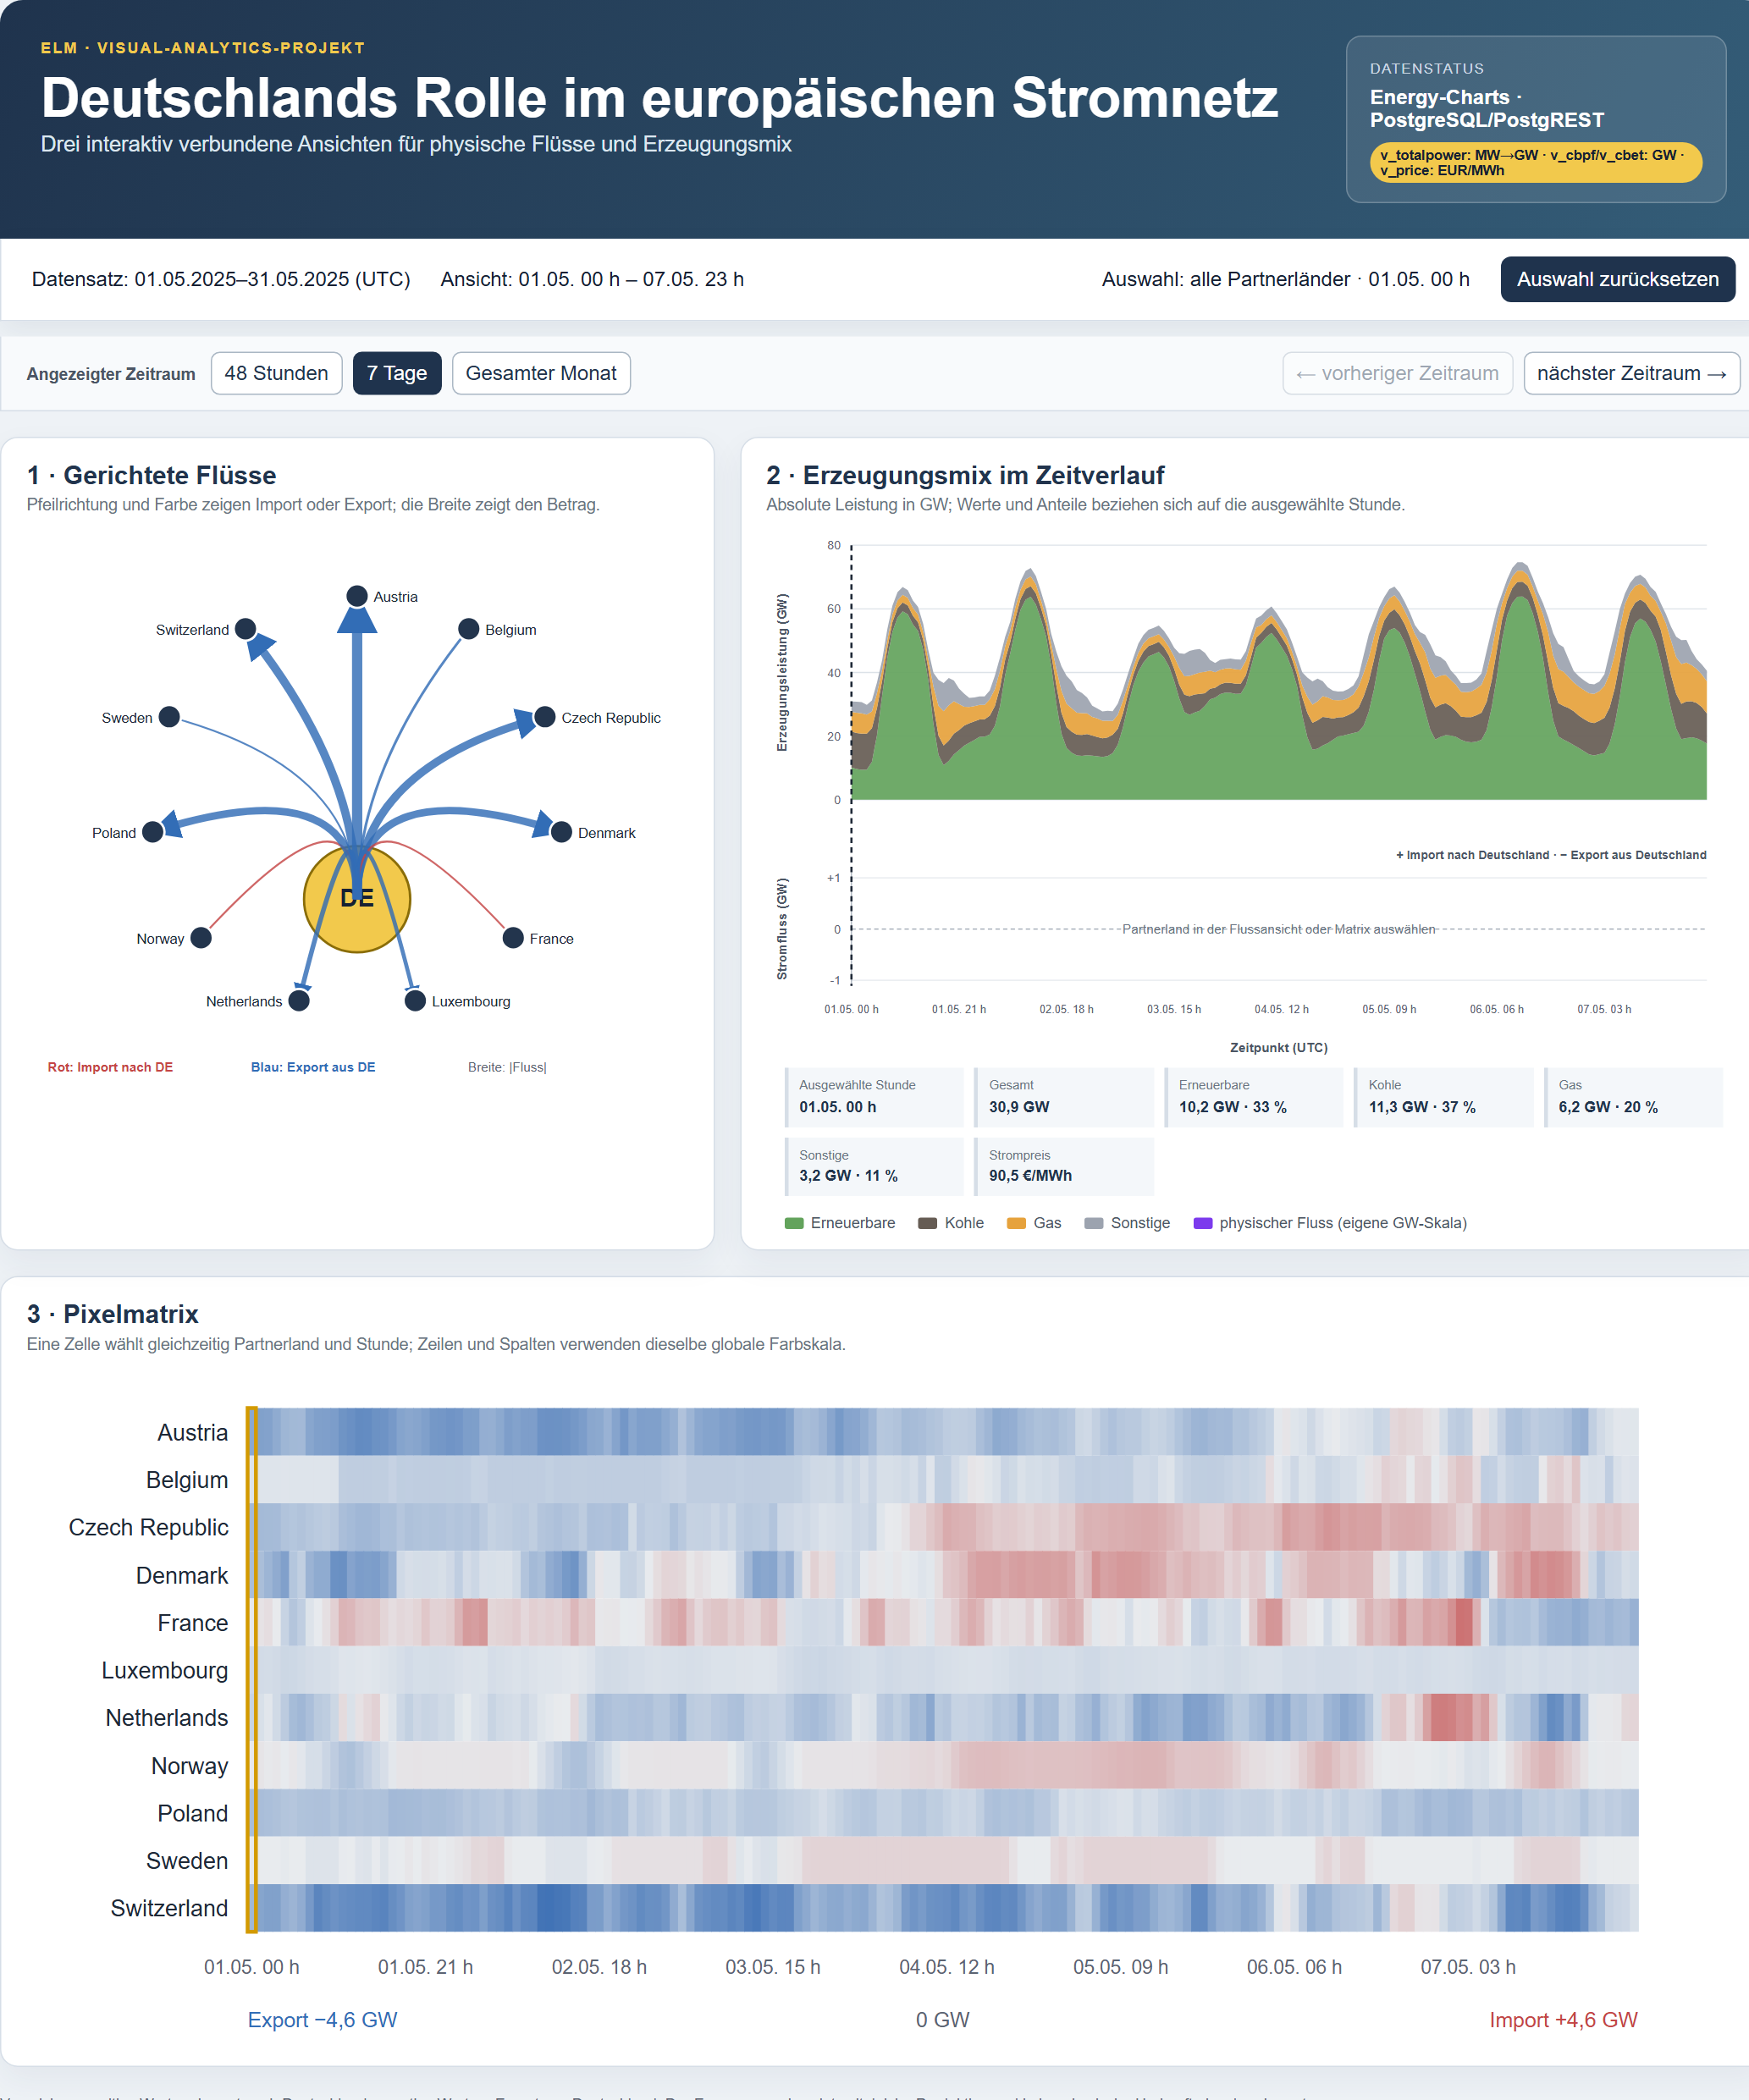
\includegraphics[width=\textwidth,height=0.79\textheight,keepaspectratio]{01_uebersicht.png}
  \caption{Gesamtansicht der Elm-Anwendung mit Netzwerk, Zeitreihe und
    Pixelmatrix. Alle Zahlen und SVG-Geometrien werden von Elm aus dem
    HTTP-Datensatz erzeugt.}
  \label{fig:overview}
\end{figure}

\subsection{Analyse der Anwendungsaufgaben}
\label{sec:aufgaben}

Aus der Forschungsfrage entstehen drei miteinander verbundene
Anwendungsaufgaben. Sie werden in \cref{tab:tasks} unabhängig von einer
konkreten Visualisierung formuliert.

\begin{table}[htbp]
  \centering
  \caption{Anwendungsaufgaben und dafür benötigte mentale Modelle.}
  \label{tab:tasks}
  \begin{tabularx}{\textwidth}{@{}p{0.08\textwidth}p{0.39\textwidth}X@{}}
    \toprule
    ID & Aufgabe & aufzubauendes mentales Modell \\
    \midrule
    A1 & Für eine Stunde erkennen, zwischen welchen Partnerländern und
      Deutschland physische Leistung in welcher Richtung und Grö{\ss}enordnung
      flie{\ss}t. & Deutschland als Zentrum eines gerichteten, gewichteten Netzes;
      Länderbeziehungen statt isolierter Tabellenzeilen. \\
    A2 & Zeitliche Muster und Ausnahmen in Erzeugungsmix, Preis und dem Fluss
      eines ausgewählten Länderpaars untersuchen. & Gemeinsame Zeitachse mit
      mehreren synchronen quantitativen Grö{\ss}en und klar getrennten Skalen. \\
    A3 & In vielen Länder-Stunden-Kombinationen Perioden mit ähnlicher Richtung,
      starken Beträgen oder Richtungswechseln finden und als Detailzustand
      auswählen. & Dichte zweidimensionale Übersicht mit Land und Zeit als
      orthogonalen Dimensionen. \\
    \bottomrule
  \end{tabularx}
\end{table}

A1 verlangt keine geografisch exakte Karte. Entscheidend ist die
Nachbarschaftsbeziehung zu Deutschland; Distanzen zwischen Ländern sind für den
Datensatz nicht definiert. A2 verlangt eine geordnete Zeitachse und quantitative
Ablesbarkeit. A3 verlangt Überblick vor Detail, weil \(744\times11=8184\)
physische Flusswerte nicht einzeln durchsucht werden sollen.

Übergreifend muss ein gefundener Zustand zwischen den mentalen Modellen
übersetzbar sein: Das in A3 entdeckte Pixel soll dasselbe Land im Beziehungsnetz
und dieselbe Stunde in der Zeitreihe aktivieren. Koordinierte Ansichten senken
diesen Übersetzungsaufwand. North und Shneiderman zeigen für
Overview-and-Detail-Kopplungen Leistungsgewinne gegenüber unkoordinierten
Ansichten \cite{north2000snap}.

\subsection{Anforderungen an die Visualisierungen}
\label{sec:anforderungen}

Aus den Aufgaben werden folgende Anforderungen abgeleitet, weiterhin ohne
einen bestimmten Diagrammtyp vorauszusetzen:

\begin{description}[style=nextline]
  \item[R1 -- Richtung und Betrag.] Positive und negative Flüsse müssen
    unterscheidbar sein; der Betrag soll zusätzlich quantitativ oder zumindest
    ordinal ablesbar bleiben.
  \item[R2 -- Länderidentität.] Alle elf Partner müssen gleichzeitig erkennbar
    und einzeln auswählbar sein.
  \item[R3 -- gemeinsame Zeit.] Erzeugung, Preis und Länderfluss müssen auf
    denselben Stundenschritt bezogen werden können.
  \item[R4 -- absolute und relative Werte.] Die Anwendung muss Leistung in GW,
    Preis in EUR/MWh und Erzeugungsanteile anzeigen, ohne unvereinbare Einheiten
    auf eine gemeinsame Achse zu zwingen.
  \item[R5 -- skalierbarer Überblick.] Ein voller Monat muss als Musterfläche
    betrachtbar sein; für genaues Ablesen sind kleinere Zeitfenster nötig.
  \item[R6 -- vergleichbare Kodierung.] Gleiche Farben müssen über Länder und
    Zeitfenster dieselbe Bedeutung besitzen. Neutrale Werte dürfen nicht wie
    fehlende Daten aussehen.
  \item[R7 -- verknüpfte Selektion.] Jede Auswahl muss sichtbar sein und die
    anderen Ansichten in einen konsistenten Zustand versetzen.
  \item[R8 -- semantische Transparenz.] Einheit, Vorzeichen, Quelle und
    Unsicherheiten müssen in der Oberfläche oder unmittelbar im Bericht
    erklärt werden.
\end{description}

\subsection{Präsentation der Visualisierungen}
\label{sec:praesentation}

\subsubsection{Visualisierung Eins: gerichteter radialer Netzwerkgraph}
\label{sec:vis1}

Deutschland bildet den zentralen Knoten, elf Partnerländer liegen radial um
ihn. Jede Kante ist gerichtet und gewichtet. Rot plus Pfeil nach Deutschland
steht für Import; Blau plus Pfeil vom Zentrum steht für Export. Richtung wird
damit redundant durch Geometrie und Farbe kodiert. Die Linienbreite bildet den
absoluten CBPF-Betrag ab. Ein Tooltip ergänzt den exakten physischen und den
kommerziellen Wert.

Diese Darstellung erfüllt A1 und R1--R2 direkt: Beziehungen sind wichtiger als
eine geografische Position, und alle Partner sind gleichzeitig sichtbar. Die
Längen der Kanten tragen keine Datenbedeutung. Dadurch wird vermieden, dass
eine schematische Länderposition als reale Leitungslänge interpretiert wird.
Im Feedback zum zweiten Zwischenstand wirkten Pfeilspitzen zu gro{\ss} und starke
Flüsse zu wenig differenziert. Die Marker wurden deshalb von 6 auf 4
SVG-Einheiten verkleinert; die maximal mögliche Linienbreite wurde deutlich
erhöht.

Eine Europakarte wäre eine echte Alternative: Sie unterstützt geografische
Orientierung und könnte reale Grenzlagen zeigen. Für nur elf Beziehungen zu
einem Zentrum benötigt sie jedoch mehr Fläche, und lange Landesnamen sowie
kleine Länder erschweren Auswahl und Beschriftung. Eine Tabelle wäre genauer,
verliert aber das gerichtete Beziehungsmodell. Der radiale Graph priorisiert
daher strukturellen Überblick, während Tooltips die exakte Zahl liefern.

\subsubsection{Visualisierung Zwei: gestapelte Zeitreihe mit Flussdetail}
\label{sec:vis2}

Vier gestapelte Flächen zeigen die absolute Erzeugungsleistung in GW. Die
linke Y-Achse beginnt bei null und wird aus dem sichtbaren Fenster auf einen
lesbaren Maximalwert gerundet. Ein darunterliegender, zeitlich ausgerichteter
Teilplot zeigt den CBPF-Wert des ausgewählten Partnerlands auf einer eigenen
symmetrischen GW-Skala. Eine gestrichelte Vertikale verbindet beide Teilplots.
Die Beschriftung ``+ Import nach Deutschland, -- Export aus Deutschland''
erklärt das Vorzeichen sichtbar.

Die Trennung der Skalen ist wesentlich: Erzeugungsleistungen von mehreren
Zehner-GW und bilaterale Flüsse von wenigen GW wären auf derselben Achse nicht
gleichzeitig lesbar. Die gemeinsame X-Achse erfüllt dennoch R3. Unter dem SVG
stehen für die ausgewählte Stunde Gesamtleistung, absolute Gruppenwerte,
Anteile, Preis und Länderfluss. So erfüllt die Ansicht R4, ohne den
Day-Ahead-Preis als fachlich unpassende zweite Linie auf die Leistungsachse zu
legen. Grundprinzipien zeitbezogener Datenvisualisierung sind ausführlich bei
Aigner et al. beschrieben \cite{aigner2011time}.

Als Alternative wäre ein 100-Prozent-Flächendiagramm geeignet, Anteile zu
vergleichen. Es würde aber absolute Produktionsspitzen verbergen. Mehrere
Small-Multiple-Linien wären für Einzeltechnologien präziser, erschweren jedoch
das Ablesen der Gesamtleistung und benötigen mehr vertikale Fläche. Die
gewählte Kombination zeigt den Gesamtumfang und die Zusammensetzung; die
Detailkarten kompensieren das schwierigere Ablesen mittlerer Stapelschichten.

\subsubsection{Visualisierung Drei: Pixelmatrix}
\label{sec:vis3}

Die Pixelmatrix ordnet Partnerländer zeilenweise und Stunden spaltenweise an.
Jede Zelle verwendet eine divergierende Farbskala: gesättigtes Blau bedeutet
starken Export, gesättigtes Rot starken Import, Hellgrau liegt nahe null. Eine
einzige globale Grenze wird aus allen 8184 CBPF-Werten des Monats berechnet.
Deshalb ist ein Rotton in der Frankreich-Zeile quantitativ mit demselben Ton in
der Dänemark-Zeile und in jedem Zeitfenster vergleichbar. Die Legende benennt
beide Skalenenden in GW.

Die Matrix erfüllt A3 sowie R5--R6. Pixelorientierte Verfahren nutzen die
Bildfläche effizient, weil jeder Messwert auf ein kleines farbiges Element
abgebildet wird \cite{keim2000pixel}. Im zweiten Zwischenstand trennten wei{\ss}e
Konturen die Zellen. Sie wurden entfernt, da Wei{\ss} sonst wie fehlende Daten
wirken und schmale Muster zerschneiden konnte. Der neutrale Bereich ist jetzt
bewusst hellgrau. Bei einer Auswahl markieren goldene Konturen die vollständige
Zeile und Spalte; die aktive Zelle erhält zusätzlich eine dunkle Kontur.

Elf übereinandergelegte Linien wären eine Alternative, erzeugten aber viele
Überdeckungen und machten Ländervergleiche schwierig. Small Multiples mit elf
separaten Linien böten bessere quantitative Ablesbarkeit, benötigten jedoch
deutlich mehr Fläche. Die Pixelmatrix ist als Überblick und Auswahlwerkzeug
konzipiert; exakte Werte werden nach Auswahl in Tooltip, Zeitreihe und
Detailkarten gelesen.

\subsection{Interaktion}
\label{sec:interaktion}

Die Kopplung folgt einem gemeinsamen Elm-Zustand. Ein Landklick im Netzwerk
aktualisiert die Partnerauswahl; die Matrixzeile wird hervorgehoben und der
untere Zeitreihenplot erscheint. Ein Klick auf die Zeitreihe aktualisiert die
Zeitwahl; Netzwerkwerte, vertikale Markierung und Matrixspalte wechseln
gleichzeitig. Eine Matrixzelle setzt beide Werte in einem Schritt.
Diese Operation bietet einen zusätzlichen Vorteil gegenüber der ohnehin
gemeinsamen X-Achse: Sie wählt zugleich eine von elf Länderdimensionen und eine
Stunde.

Die sichtbaren Zeitfenster 48 Stunden, sieben Tage und gesamter Monat erfüllen
R5. Vor- und Zurück-Schaltflächen verschieben kleinere Fenster ohne
Datenüberlauf. Beim Fensterwechsel bleibt die Partnerwahl erhalten; die
Zeitwahl wird auf einen gültigen Index gesetzt. ``Auswahl zurücksetzen'' löscht
den Länderfilter und setzt die Zeit an den Beginn des aktuellen Fensters.

Nicht umgesetzt wurden freies Zoomen, Mehrfachauswahl und Sortieren der
Matrixzeilen. Sie würden zusätzliche Zustände und Konflikte erzeugen, ohne für
die drei Kernaufgaben nötig zu sein. Die feste Reihenfolge erleichtert
Vergleiche zwischen Fenstern; drei wohldefinierte Zeitskalen sind für den
Monatsdatensatz verständlicher als ein unbeschrifteter Zoomfaktor.

\section{Implementierung}
\label{sec:implementierung}

\subsection*{Gesamtaufbau}

Die Webanwendung ist mit Elm~0.19.1 implementiert und erzeugt alle drei
Visualisierungen als SVG. Sie folgt The Elm Architecture mit den Schritten
Model, View und Update \cite{elmArchitecture}. \Cref{fig:architecture} zeigt
den Daten- und Zustandsfluss.

\begin{figure}[htbp]
  \centering
  \begin{tikzpicture}[
    node distance=11mm and 13mm,
    box/.style={draw=projectblue,rounded corners,fill=blue!3,minimum width=35mm,minimum height=9mm,align=center},
    arrow/.style={-{Latex[length=2.5mm]},thick,draw=projectblue}
  ]
    \node[box] (json) {\code{public/data/energy.json}\\744 Stunden per HTTP};
    \node[box,below=of json] (api) {\code{Api.elm}\\Decoder und Fehlerzustand};
    \node[box,below=of api] (main) {\code{Main.elm}\\Model, Update, Zeitfenster};
    \node[box,below left=of main] (network) {\code{FlowNetwork.elm}\\Land wählen};
    \node[box,below=of main] (time) {\code{TimeSeries.elm}\\Stunde wählen};
    \node[box,below right=of main] (matrix) {\code{FlowMatrix.elm}\\Land und Stunde wählen};
    \draw[arrow] (json) -- (api);
    \draw[arrow] (api) -- (main);
    \draw[arrow] (main) -- (network);
    \draw[arrow] (main) -- (time);
    \draw[arrow] (main) -- (matrix);
    \draw[arrow,bend left=18] (network) to (main);
    \draw[arrow,bend right=18] (time) to (main);
    \draw[arrow,bend right=28] (matrix) to (main);
  \end{tikzpicture}
  \caption{Modulstruktur und gerichteter Datenfluss der Elm-Anwendung.}
  \label{fig:architecture}
\end{figure}

Das Modul \code{Domain.elm} enthält die fachlichen Typen. \code{Api.elm}
lädt und decodiert den normalisierten Datensatz per HTTP. Die Views sind
zustandslos: Sie erhalten Daten und Callback-Funktionen, erzeugen SVG und senden
bei Interaktion eine Nachricht an \code{Main.elm}. Dadurch können die drei
Ansichten nicht unbemerkt auseinanderlaufen.

\subsection*{Wichtigste Elm-Datenstrukturen}

Der globale Zustand nach erfolgreichem Laden lautet verkürzt:

\begin{lstlisting}[language={}]
type alias State =
    { dataset : Dataset
    , selectedIndex : Int
    , selectedPartner : Maybe String
    , windowStart : Int
    , windowSize : Int
    }
\end{lstlisting}

\code{selectedIndex} ist ein globaler Index in den 744 Stunden. Für jede View
wird daraus ein lokaler Index des sichtbaren Fensters gebildet.
\code{selectedPartner} ist optional, weil die Erzeugungszeitreihe auch ohne
Länderfilter sinnvoll bleibt. \code{windowStart} und \code{windowSize}
definieren 48-Stunden-, 7-Tage- oder Monatsansicht.

Die wichtigsten Nachrichten sind:

\begin{lstlisting}[language={}]
type Msg
    = GotDataset (Result Http.Error Dataset)
    | SelectPartner String
    | SelectTime Int
    | SelectCell String Int
    | SetWindowSize Int
    | MoveWindow Int
    | Reset
\end{lstlisting}

\code{SelectCell} setzt Partner und Zeit atomar. \code{MoveWindow} begrenzt
den neuen Start mit \code{clamp}; dadurch kann weder vor den ersten noch hinter
den letzten Datensatz gesprungen werden. Ladefehler erzeugen einen sichtbaren
Fehlerzustand statt einer leeren Seite.

\subsection*{SVG-Berechnung}

Der Netzwerkgraph berechnet Positionen auf einem Kreis aus Index und Anzahl der
Partner. Ein quadratischer Bézier-Pfad verbindet jeden Partner mit dem
deutschen Knoten. Das Vorzeichen bestimmt Reihenfolge der Endpunkte,
Pfeilmarker und Farbe; \(1{,}5+\min(20,3{,}2|x|)\) bestimmt die Linienbreite.

Die Zeitreihe summiert für jede Stunde die vier Gruppen. Für jede gestapelte
Fläche wird eine obere und untere Punktfolge zu einem geschlossenen SVG-Pfad
verbunden. Die Y-Skala wird aus dem Maximalwert des sichtbaren Fensters und
einer gerundeten Schrittweite bestimmt. Der Länderfluss besitzt eine getrennte
symmetrische Skala. Über jedem Stundenintervall liegt ein transparenter
Trefferbereich, sodass die Auswahl nicht auf eine dünne Linie beschränkt ist.

Die Pixelmatrix berechnet die Zellbreite aus Fensterlänge und verfügbarer
Breite. Der Betrag wird durch das globale Maximum aller Monatswerte normiert;
danach wird zwischen Hellgrau und Rot beziehungsweise Blau linear interpoliert.
Die Farbnorm hängt somit nicht vom sichtbaren Fenster ab.

\subsection*{Implementierungsaufwand und Entscheidungen}

Relativ direkt war die Umsetzung des Elm-Grundgerüsts, der JSON-Decoder und
einfacher SVG-Elemente auf Basis der Übungen. Aufwändiger waren die
Vorverarbeitung heterogener View-Schemata, die korrekte Einheit von
\code{v\_totalpower}, das Paginieren von mehr als 1000 Rohzeilen, gestapelte
Flächenpfade, zwei quantitative Y-Skalen und die Umrechnung zwischen globalem
und lokalem Zeitindex.

Eine direkte Authentifizierung aus Elm wurde verworfen. Das Passwort müsste in
einer öffentlichen Pages-Anwendung eingegeben oder der Token sichtbar werden.
Stattdessen trennt die Pipeline geschützten Export und öffentliche Analyse. Die
fertige JSON-Datei wird dennoch per HTTP geladen und kann unabhängig vom
Entwicklungsrechner ausgeliefert werden.

\subsection*{Prüfung und Bereitstellung}

Der Produktionsbuild wurde mit folgendem Befehl erfolgreich erzeugt:

\begin{lstlisting}[language={}]
elm make src/Main.elm --optimize --output=public/elm.js
\end{lstlisting}

Ein automatisches Prüfskript validiert Datenumfang, lückenlose Stundenschritte,
Partnerabdeckung und Wertebereiche. Im Browser wurden alle Auswahlpfade sowie
Zeitraumwechsel manuell ausgeführt. Neue JavaScript- oder HTTP-Fehler traten im
optimierten Build nicht auf. Ein reproduzierbares Capture-Skript wiederholt
definierte Klickfolgen über das Browser-Debug-Protokoll. So entstehen die
Berichtsabbildungen direkt aus der laufenden Elm-Anwendung.

Die Datei \code{.gitlab-ci.yml} verwendet ein Node-Abbild, installiert die
fixierte Elm-Version~0.19.1-6, kompiliert mit \code{--optimize} und publiziert
den Ordner \code{public} über GitLab Pages. Quellcode und Anwendung liegen im
\projectlink{öffentlichen Hochschul-GitLab-Projekt}. Die lokale Git-Historie
ist im Anhang dokumentiert.

\subsection*{Einsatz von KI}

Für Entwürfe von Elm-Code, Python-Hilfsskripten, Dokumentation und Bericht wurde
ausschlie{\ss}lich OpenAI Codex verwendet. Themenwahl, Rückfragen, fachliche
Prioritäten und Abnahme lagen beim Verfasser. KI-Ausgaben wurden nicht ungeprüft
übernommen: Der Code wurde kompiliert, Daten wurden mit unabhängigen
Validierungsregeln geprüft, Interaktionen im Browser ausgeführt und jede Seite
des erzeugten PDF visuell kontrolliert. Fehler und unklare Annahmen führten zu
weiteren Prompts und Änderungen. Die relevanten Nutzereingaben sind nach
Programmteil in \cref{app:ki} aufgeführt; KI-Ausgaben werden entsprechend der
Vorgabe nicht wiederholt.

\section{Anwendungsfälle}
\label{sec:anwendungsfaelle}

Die folgenden Fälle zeigen jeweils einen fachlich interpretierbaren Befund und
den dafür benötigten Interaktionsweg. Die drei Zustände sind keine zwingende
lineare Klickfolge: Für jeden Fall wird die passende Zeitspanne gewählt. So
führt der Dänemark-Zustand in \cref{sec:case3} nicht versehentlich den zuvor
gewählten Frankreich-Zustand fort, sondern demonstriert einen unabhängigen
Einstieg über die Matrix.

\subsection{Anwendung Visualisierung Eins}
\label{sec:case1}

Ausgangspunkt ist der 1. Mai 2025 um 00 Uhr UTC. Ein Klick auf Frankreich im
gerichteten Netzwerk wählt das Länderpaar. In \cref{fig:case-france} sind
Frankreichs Knoten gelb und seine Kante kräftig, während die übrigen Kanten
abgeblendet sind. Die rote Pfeilrichtung zeigt einen kleinen physischen Import
von Frankreich nach Deutschland (\(+0{,}058\gw\)). Der Tooltip nennt zugleich
einen Handelswert von \(-2{,}940\gw\), also kommerziellen Export in der hier
verwendeten Vorzeichenkonvention.

\begin{figure}[htbp]
  \centering
  \begin{tikzpicture}
    \node[anchor=south west,inner sep=0] (img) at (0,0)
      {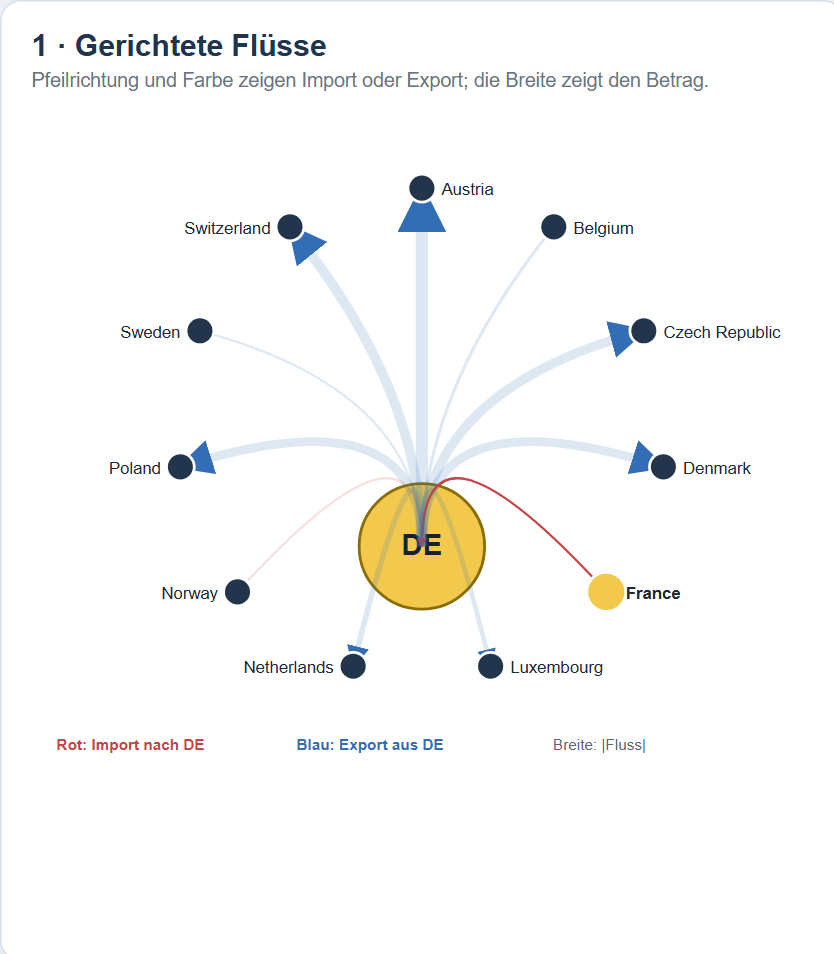
\includegraphics[width=0.70\textwidth]{02_frankreich_netzwerk.png}};
    \begin{scope}[x={(img.south east)},y={(img.north west)}]
      \draw[importred,very thick,-{Latex[length=3mm]}]
        (0.91,0.68) node[above left,fill=white,rounded corners,inner sep=2pt,
          text=importred,font=\sffamily\bfseries\small]{1: gewählte Beziehung}
        -- (0.735,0.385);
      \draw[projectyellow!70!black,very thick]
        (0.735,0.38) circle[radius=0.032];
    \end{scope}
  \end{tikzpicture}
  \caption{Frankreich ist ausgewählt. Knoten und Kante bleiben hervorgehoben;
    die rote Richtung steht für physischen Import nach Deutschland.}
  \label{fig:case-france}
\end{figure}

Der Befund ist für die Zielgruppe wichtig, weil er unmittelbar zeigt, warum
Handel und physischer Fluss nicht synonym verwendet werden dürfen. Eine Tabelle
könnte die beiden exakten Werte sogar schneller liefern, würde aber nicht
gleichzeitig sichtbar machen, wie schwach die ausgewählte physische Kante im
Vergleich zu starken Exportkanten nach Österreich, in die Schweiz oder nach
Polen ist. Der Netzwerkgraph liefert den relationalen Kontext; der Tooltip
liefert die Präzision.

\subsection{Anwendung Visualisierung Zwei}
\label{sec:case2}

Für die Woche vom 8. bis 14. Mai wird Frankreich gewählt und anschlie{\ss}end der
11. Mai 2025 um 11 Uhr UTC angeklickt. Die gestrichelte Vertikale in
\cref{fig:case-price} verbindet Erzeugungsmix und Frankreich-Fluss. In dieser
Stunde beträgt die erneuerbare Leistung \(58{,}961\gw\), entsprechend
88,7\,\% der dargestellten Gesamterzeugung von etwa \(66{,}5\gw\). Der
Day-Ahead-Preis erreicht mit \(-250{,}32\mwh\) das Monatsminimum, während aus
Frankreich physisch \(+1{,}382\gw\) importiert werden.

\begin{figure}[htbp]
  \centering
  \begin{tikzpicture}
    \node[anchor=south west,inner sep=0] (img) at (0,0)
      {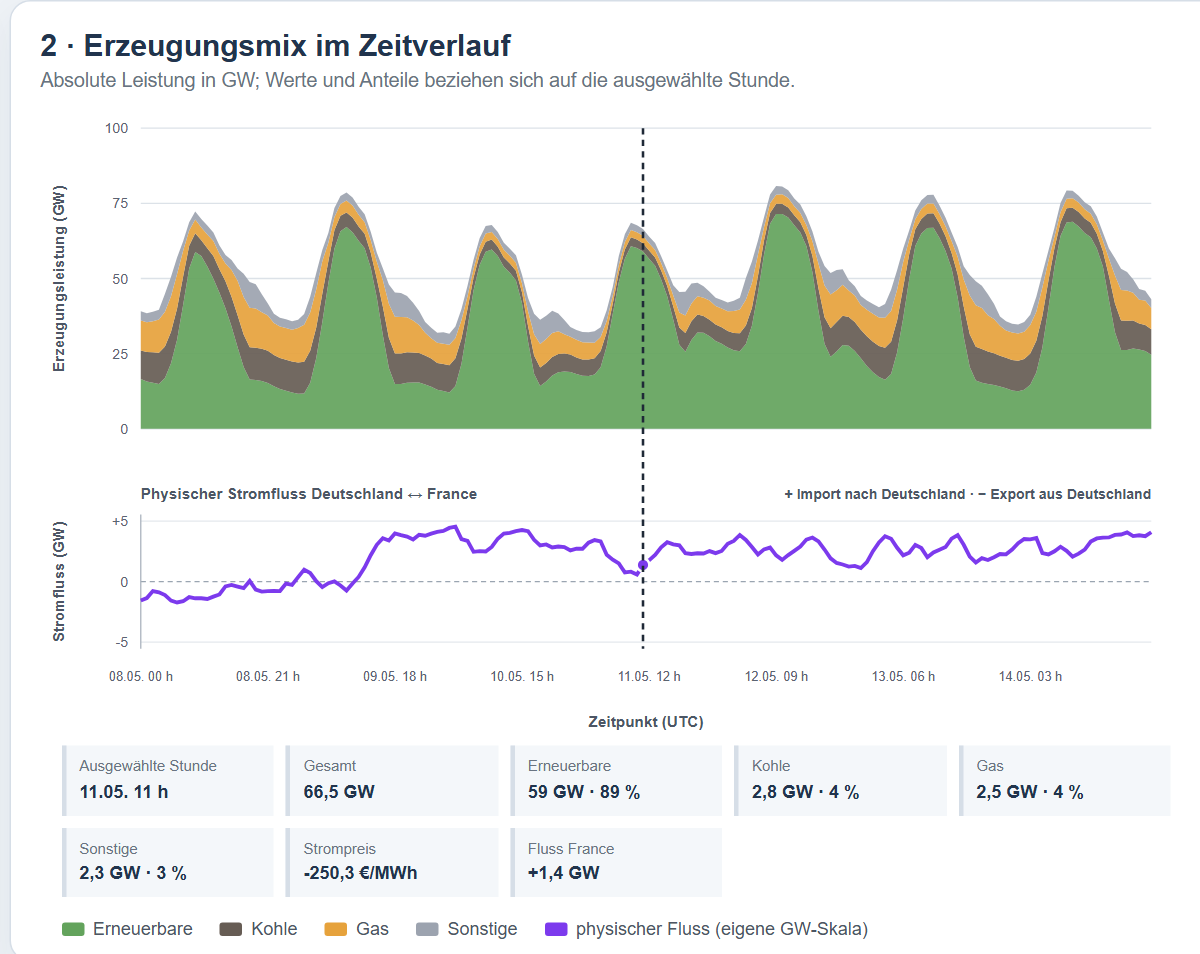
\includegraphics[width=0.98\textwidth]{03_negativpreis_zeitreihe.png}};
    \begin{scope}[x={(img.south east)},y={(img.north west)}]
      \draw[importred,very thick,-{Latex[length=3mm]}]
        (0.69,0.96) node[below,fill=white,rounded corners,inner sep=2pt,
          text=importred,font=\sffamily\bfseries\small]{1: gewählte Stunde}
        -- (0.535,0.69);
      \draw[projectblue,very thick,-{Latex[length=3mm]}]
        (0.87,0.90) node[below,fill=white,rounded corners,inner sep=2pt,
          text=projectblue,font=\sffamily\bfseries\small]{2: Preis und Absolutwerte}
        -- (0.535,0.17);
    \end{scope}
  \end{tikzpicture}
  \caption{Monatliches Preisminimum. Die gemeinsame Zeitmarke verbindet
    erneuerbare Erzeugung, Frankreich-Fluss und Detailwerte.}
  \label{fig:case-price}
\end{figure}

\FloatBarrier

Über den ganzen Mai korreliert der Preis mit der absoluten erneuerbaren
Leistung mit \(r=-0{,}758\), mit ihrem Anteil sogar mit \(r=-0{,}817\). Dies
ist ein sichtbares und statistisch gestütztes Monatsmuster, aber kein
Kausalnachweis. Der einfache summierte physische Fluss korreliert dagegen nur
mit \(r=0{,}084\) mit dem Preis. Die Anwendung verhindert damit eine zu einfache
Erzählung ``mehr Export erklärt negative Preise'': Der konkrete Länderfluss,
andere Erzeugungsarten, Nachfrage, Netzrestriktionen und Markteffekte können
abweichen.

Ein Scatterplot von Preis und erneuerbarer Leistung wäre für die Korrelation
präziser und ist eine sinnvolle spätere Ergänzung. Er würde jedoch die
Reihenfolge der Stunden, Tagesmuster und den zeitgleichen Frankreich-Fluss
verbergen. Für die Untersuchung eines Ereignisverlaufs ist die gekoppelte
Zeitreihe geeigneter; für einen globalen Zusammenhang wäre der Scatterplot
effizienter.

\subsection{Anwendung Visualisierung Drei}
\label{sec:case3}

Nach Rückkehr zum 48-Stunden-Fenster 3.--4. Mai wird die Matrixzelle Dänemark,
3. Mai um 12 Uhr angeklickt. \Cref{fig:case-matrix} markiert die vollständige
Dänemark-Zeile und die 12-Uhr-Spalte als Fadenkreuz. Die aktive Zelle zeigt
einen Export aus Deutschland von \(-1{,}710\gw\). In derselben Spalte sind
auch Österreich, Belgien, Tschechien, Luxemburg, Niederlande, Norwegen, Polen,
Schweden und Schweiz blau oder nahe neutral, während Frankreich rötlich ist
(\(+0{,}582\gw\) Import).

\begin{figure}[htbp]
  \centering
  \begin{tikzpicture}
    \node[anchor=south west,inner sep=0] (img) at (0,0)
      {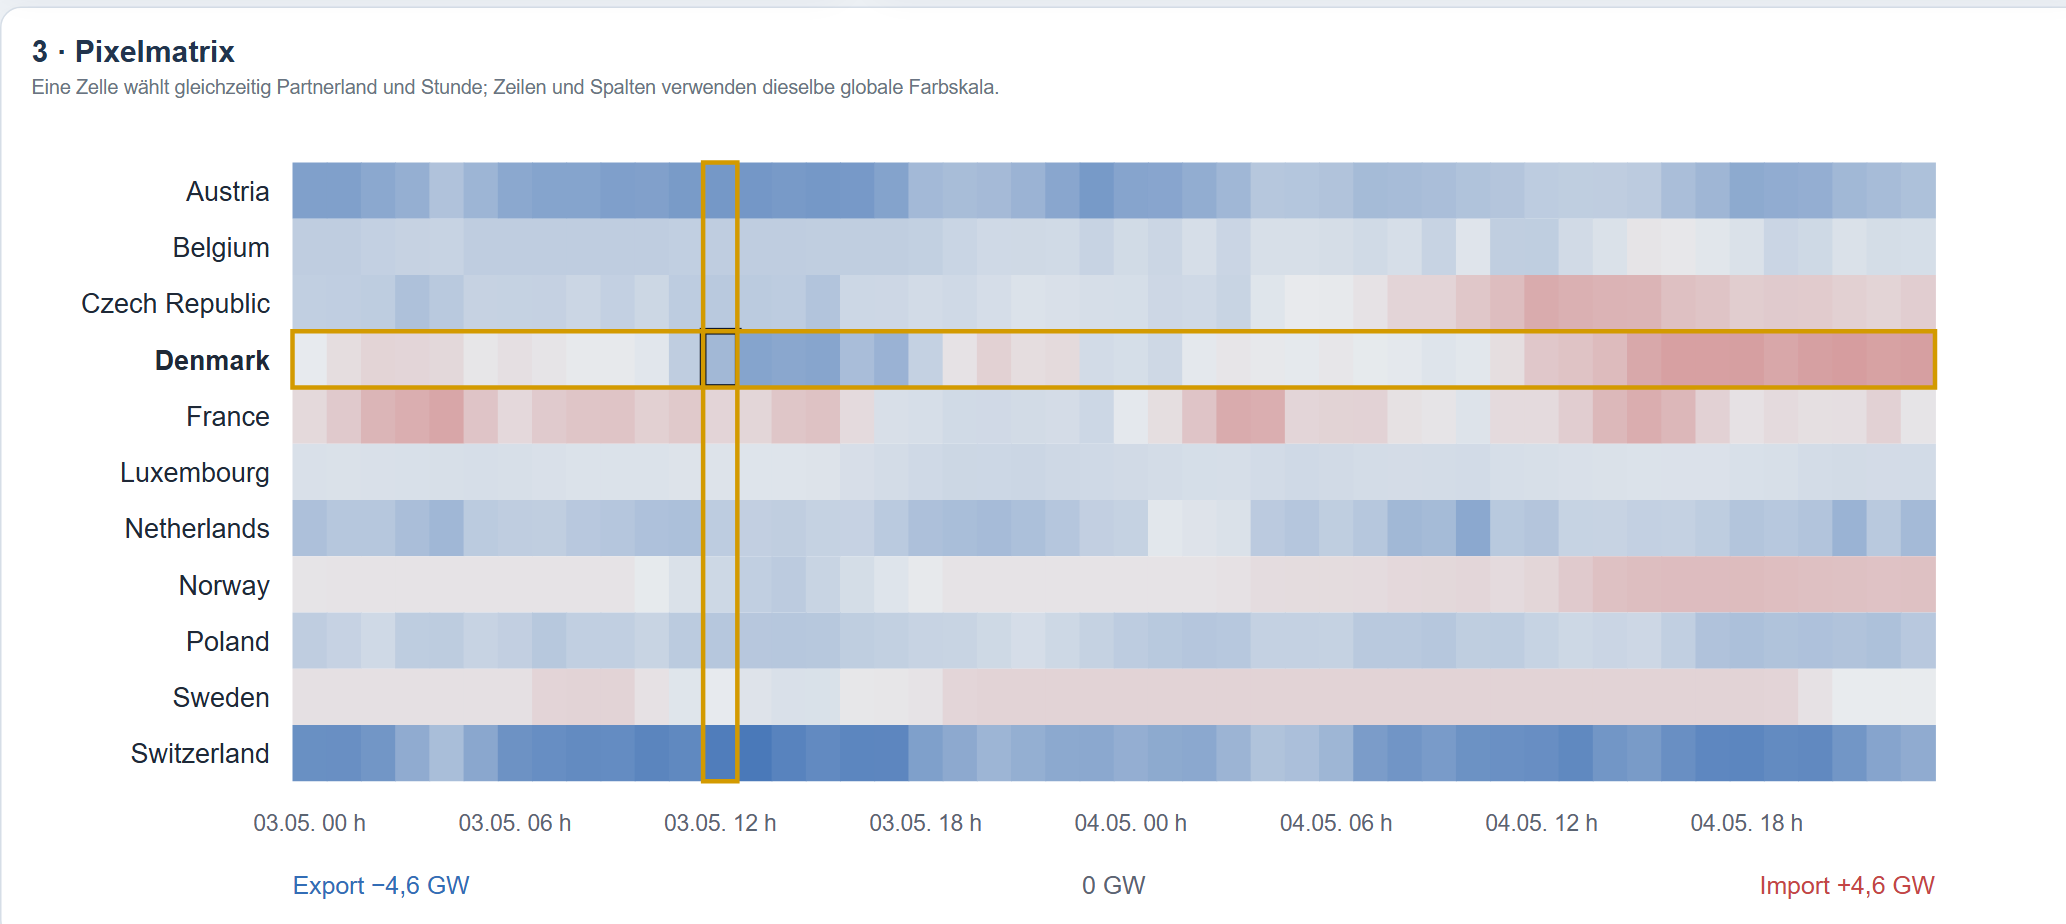
\includegraphics[width=\textwidth]{04_daenemark_matrix.png}};
    \begin{scope}[x={(img.south east)},y={(img.north west)}]
      \draw[importred,very thick,-{Latex[length=3mm]}]
        (0.14,0.93) node[right,fill=white,rounded corners,inner sep=2pt,
          text=importred,font=\sffamily\bfseries\small]{1: Partnerzeile}
        -- (0.30,0.62);
      \draw[projectblue,very thick,-{Latex[length=3mm]}]
        (0.50,0.94) node[right,fill=white,rounded corners,inner sep=2pt,
          text=projectblue,font=\sffamily\bfseries\small]{2: Stunde}
        -- (0.346,0.62);
    \end{scope}
  \end{tikzpicture}
  \caption{Auswahl der Zelle Dänemark, 03.05.2025 12 Uhr UTC. Das goldene
    Fadenkreuz macht beide gewählten Dimensionen sichtbar.}
  \label{fig:case-matrix}
\end{figure}

\FloatBarrier

Die visuelle Aufgabe besteht nicht nur darin, einen Einzelwert abzulesen,
sondern das gleichzeitige Länderprofil zu sehen. Das Muster legt nahe, dass der
deutsche physische Austausch in dieser Stunde gegenüber vielen Partnern in
Exportrichtung verlief, aber nicht gegenüber Frankreich. Die globale Farbskala
macht die Sättigungen zeilenübergreifend vergleichbar. Eine Tabelle wäre für
den Wert \(-1{,}710\gw\) genauer, verlangte für das Profil jedoch serielles
Lesen von elf Zeilen. Elf Linien hätten stärkere Überdeckung. Die Matrix
unterstützt das parallele Erkennen, die gekoppelten Detailansichten übernehmen
die quantitative Prüfung.

\FloatBarrier

\section{Verwandte Arbeiten}
\label{sec:related}

Steiger et al. verbinden ein regelbasiertes Expertensystem mit mehreren
koordinierten Ansichten für die Überwachung eines Smart Grids
\cite{steiger2013smartgrid}. Eine Übersicht zeigt Zustände verteilter
Netzelemente; eine Analyseansicht macht den Verarbeitungspfad von Alarmen
nachvollziehbar. Gemeinsam mit diesem Projekt sind der Energiekontext,
Details-on-Demand und die Selektion eines Elements, die eine zweite Ansicht
aktualisiert. Der Unterschied liegt im Analyseziel: Steiger et al. unterstützen
operative Störungsdiagnose und erklären automatische Regeln. Die vorliegende
Anwendung arbeitet retrospektiv mit länderbezogenen Flüssen, Erzeugung und
Preis; sie enthält weder Alarmmodell noch Handlungsempfehlung.

Jäger et al. untersuchen die Kombination topologischer und geografischer
Information für das Management elektrischer Ausfälle
\cite{jaeger2016outage}. Ihre Designstudie zeigt, dass getrennte Räume einen
mentalen Abgleich verlangen, und nutzt interaktives Brushing-and-Linking. Das
stützt die Entscheidung, Länderbeziehung und Zeitmuster koordiniert zu zeigen.
Anders als dort ist Geografie für die Projektaufgabe keine zwingende
Datendimension: Die Abstände und Formen der Länder erklären weder Flussbetrag
noch Handel. Deshalb ersetzt ein kompakter radialer Graph die Kartenansicht.
Eine künftige Erweiterung könnte eine Karte ergänzen, wenn reale
Grenzkuppelleitungen und räumliche Engpässe einbezogen werden.

AMPLIO VQA von Stoffel et al. analysiert Simulationen für die Planung eines
Microgrid-Erzeugungsmixes \cite{stoffel2012amplio}. Beide Systeme behandeln
mehrdimensionale zeitbezogene Energiedaten und kombinieren Überblick,
Interaktion und Detail. AMPLIO vergleicht jedoch parametrisierte
Planungsszenarien und unterstützt visuelle Anfragen; dieses Projekt untersucht
gemessene historische Daten und einen nationalen grenzüberschreitenden
Austausch. Die gestapelte Zeitreihe ähnelt dem gemeinsamen Bedarf, einen Mix
über Zeit zu verstehen, während Netzwerk und Pixelmatrix speziell aus den
Dimensionen Partnerland und Stunde abgeleitet sind.

Methodisch steht die Anwendung in der Tradition koordinierter multipler
Ansichten. North und Shneiderman beschreiben Koordination als Grundlage für
Brushing-and-Linking und Overview-and-Detail \cite{north2000snap}. Die
vorliegende Implementierung erlaubt Nutzenden zwar nicht, Ansichten frei zu
konfigurieren, realisiert aber eine feste, domänenspezifische Kopplung über
Land und Zeit. Die Pixelmatrix folgt dem Prinzip pixelorientierter Techniken,
möglichst viele Einzelwerte gleichzeitig auf Bildschirmfläche abzubilden
\cite{keim2000pixel}; anders als allgemeine hochdimensionale Verfahren nutzt
sie eine fachlich feste Ordnung der Achsen.

Insgesamt unterscheidet sich das Projekt von den drei Energiearbeiten durch
die konkrete Kombination aus bilateralem Ländergraph, Erzeugungs-/Flusszeitreihe
und Länder-Stunden-Matrix auf realen Energy-Charts-Daten. Es ist kleiner und
nicht als Leitwartenwerkzeug evaluiert. Sein Beitrag liegt in einer
nachvollziehbaren, auf eine Lehr- und Explorationszielgruppe zugeschnittenen
Integration, nicht in einem neuen Visualisierungsalgorithmus.

\section{Zusammenfassung und Ausblick}
\label{sec:fazit}

Das Projekt beantwortet die Ausgangsfrage nicht mit einer einzelnen Kennzahl,
sondern mit einem nachvollziehbaren Analyseweg. Der gerichtete Netzwerkgraph
zeigt Deutschlands bilaterale Rolle zu einer Stunde. Die gestapelte Zeitreihe
verbindet absolute Erzeugung, relative Anteile, Preis und einen ausgewählten
Länderfluss. Die Pixelmatrix verdichtet 8184 physische Flusswerte zu einem
Überblick und dient zugleich als zweidimensionales Auswahlwerkzeug. Ein
gemeinsamer Elm-Zustand hält Land, Stunde und Zeitfenster konsistent.

Für den Mai 2025 zeigt die Fallanalyse deutliche Preisunterschiede und einen
starken negativen linearen Zusammenhang zwischen Preis und erneuerbarer
Leistung. Gleichzeitig ist der Zusammenhang zwischen Preis und einfacher Summe
der bilateralen physischen Flüsse schwach. Einzelne Länderbeziehungen können
zudem kommerziell und physisch verschiedene Richtungen aufweisen. Damit liefert
die Anwendung einen echten Mehrwert: Sie macht einfache Erklärungen prüfbar und
führt von einem Muster unmittelbar zu konkreten absoluten Werten.

Sinnvolle Erweiterungen sind:

\begin{itemize}
  \item frei wählbare Start- und Enddaten sowie serverseitig erzeugte Exporte,
  \item Drill-down von den vier Gruppen zu einzelnen Erzeugungstechnologien,
  \item ein ergänzender Scatterplot für Preis--Erzeugungs-Zusammenhänge,
  \item Vergleich physischer und kommerzieller Flüsse als Differenzansicht,
  \item saisonale oder mehrjährige Aggregation mit Zoom und
        Kalender-Hierarchie,
  \item eine Nutzerstudie mit Studierenden und energiewirtschaftlich
        Vorgebildeten.
\end{itemize}

Für längere Zeiträume müsste die Matrix aggregieren oder hierarchisch zoomen;
sonst werden Stunden schmaler als wahrnehmbare Pixel. Au{\ss}erdem sollte eine
künftige Analyse Nachfrage, installierte Leistung, Wetter und Netzengpässe
einbeziehen, bevor kausale Aussagen über Preis oder Fluss entstehen. In der
aktuellen Form bleibt das System bewusst ein exploratives Werkzeug mit klar
begrenzter Aussagekraft.


\appendix
\section{Git-Historie}
\label{app:git}

Die Entwicklung wurde in getrennten lokalen Commits dokumentiert. Der folgende
Auszug wurde mit \code{git log --oneline --decorate --graph --all} erzeugt. Der
öffentliche GitLab-Stand wird erst nach ausdrücklicher Freigabe hochgeladen.

\begin{lstlisting}[language={}]
* 0b279b9 Fallstudie und reproduzierbare Abbildungen ergänzen
* 1e34819 GitLab Pages und Projektdokumentation ergänzen
* e12b666 Daten- und Interaktionstests dokumentieren
* b6c805e Visualisierungen und Zeitraumsteuerung überarbeiten
* 4376a21 Datenpipeline auf Mai 2025 erweitern
*   79f38a9 Hochschul-GitLab mit bestehender Projekthistorie verbinden
|\
| * ff86945 Initial commit
* 969d7f3 2. Zwischenstand überarbeitet
* 3882dc7 2. Abbildung detailreicher und Zwischenbericht angepasst
* 693c16b GitHub hinzugefügt
* 23c6a28 Elm code sowie Zwischenstand aktualisiert
* 2c8bada Ordnerstruktur und erste zwischenstände
\end{lstlisting}

Der Bericht gehört nach der inhaltlichen und visuellen Endprüfung zu einem
eigenen abschlie{\ss}enden Commit. Dessen Hash kann nicht Bestandteil des in
diesem Commit erzeugten PDFs sein. Der Merge-Commit \code{79f38a9} verbindet
die vorhandene Projekthistorie mit dem initialen Commit des öffentlichen
Hochschul-GitLab-Projekts, ohne frühere Arbeit zu überschreiben.

\section{KI-gestützter Arbeitsprozess}
\label{app:ki}

Dieser Anhang fasst die Zusammenarbeit mit OpenAI Codex zusammen. Er ist kein
wörtliches Gesprächsprotokoll, sondern beschreibt die schrittweise erteilten
Arbeitsaufträge und die daraus entstandenen Ergebnisse. Thema, fachliche
Prioritäten und Freigaben wurden vom Verfasser festgelegt. Codex unterstützte
bei Recherche, Implementierungsentwürfen, Prüfungen und Formulierungen; die
Zwischenergebnisse wurden jeweils betrachtet, besprochen und weiterentwickelt.

\subsection*{A: Themenwahl und Datenzugang}

\begin{enumerate}
  \item Zunächst wurden mehrere geeignete Energy-Charts-Themen gegenübergestellt.
    Danach wurde die Untersuchung von Deutschlands Importen, Exporten,
    Länderbeziehungen, Erzeugungsmix und Preisen als Leitfrage festgelegt.
  \item Anschlie{\ss}end wurden der Datenbankzugang und das bereitgestellte Schema
    \code{energycharts} geprüft. Es folgten begrenzte PostgREST-Abfragen. Dabei
    wurden Datenquelle, HTTP-Endpunkte und Zugangshinweise getrennt von den
    exportierten Analysedaten dokumentiert.
  \item Nach Rückfragen zu den Einheiten wurden die OpenAPI-Beschreibung von
    Energy-Charts und die tatsächlichen Wertebereiche geprüft. Erst danach
    wurden GW, MW, EUR/MWh und die Vorzeichenkonvention verbindlich festgelegt.
  \item Für erste Tests wurden kleine Ausschnitte geladen. Nach erfolgreicher
    Prüfung wurde die Pipeline auf den vollständigen Mai 2025 mit 744 Stunden
    und elf Partnerländern erweitert.
\end{enumerate}

\subsection*{B: Elm-Visualisierungen und Interaktion}

\begin{enumerate}
  \item Der erste Prototyp verband einen gerichteten Ländergraphen, eine
    Zeitreihe und eine Pixelmatrix. Vorläufige Python-Abbildungen wurden danach
    vollständig durch SVG-Ansichten aus Elm ersetzt; Python blieb nur für
    Datenexport und Validierung zuständig.
  \item Die Bedienung wurde gemeinsam schrittweise geprüft: Land im Netzwerk
    wählen, Stunde in der Zeitreihe setzen und Land plus Stunde über eine
    Matrixzelle auswählen. Unabhängige Anwendungsfälle wurden deutlicher
    voneinander getrennt, damit Auswahlzustände nicht als feste Klickfolge
    missverstanden werden.
  \item Bei der Besprechung des Zeitdiagramms fiel auf, dass absolute Werte und
    Skalen fehlten. Daraufhin kamen eine beschriftete GW-Y-Achse, eine eigene
    symmetrische Flussskala, absolute Detailwerte und relative Anteile hinzu.
  \item Die Professorenhinweise wurden anschlie{\ss}end als Änderungsaufgaben
    umgesetzt: kleinere Pfeile, stärkere Maximallinien, mehrere Zeitfenster,
    globale Matrixfarben, eine Nullwertfarbe ohne wei{\ss}e Lücken und sichtbarere
    Auswahlmarkierungen.
  \item Nach jedem grö{\ss}eren Schritt wurden Elm-Build, Datensatzregeln und die
    relevanten Interaktionen erneut geprüft. Die finalen Abbildungen entstanden
    reproduzierbar aus festgelegten Zuständen der laufenden Elm-Anwendung.
\end{enumerate}

\subsection*{C: Berichtsrevision und Abschluss}

\begin{enumerate}
  \item Zunächst entstanden ein knapper Projektplan und zwei bearbeitbare
    Zwischenstände. Die Rückfragen des Verfassers zu Abbildungen, Bedienung und
    Formulierungen führten jeweils zu gezielten Überarbeitungen.
  \item Für den Abschluss wurden Berichtsvorlage, Protokoll und sämtliche
    Kommentare zum zweiten Zwischenstand ausgewertet. Daraus entstand die feste
    Gliederung; die Umsetzung jeder Rückmeldung ist in Anhang~C nachvollziehbar.
  \item Quellen zu Energy-Charts, PostgREST, Elm und verwandten Arbeiten wurden
    recherchiert und als BibTeX-Einträge eingebunden. Aussagen zu Einheiten und
    Datenbedeutung wurden auf Primärquellen zurückgeführt.
  \item Text, Tabellen und annotierte Screenshots wurden anschlie{\ss}end in LaTeX
    zusammengeführt. Der Bericht wurde kompiliert, vollständig gerendert und
    Seite für Seite visuell geprüft.
  \item Änderungen an Daten, Visualisierungen, Experimenten, Dokumentation und
    Bericht wurden in getrennten lokalen Git-Commits festgehalten. Ein Upload
    in das öffentliche Hochschul-GitLab erfolgt erst nach ausdrücklicher
    Freigabe.
\end{enumerate}

\section{Umsetzung des Feedbacks zum zweiten Zwischenstand}
\label{app:feedback}

\begin{longtable}{@{}p{0.32\textwidth}p{0.62\textwidth}@{}}
  \toprule
  Rückmeldung & Umsetzung \\
  \midrule
  \endhead
  Text ausbauen; Text direkt unter ``Einleitung'' & Zielproblem und
    Forschungsfrage stehen jetzt vor Unterabschnitt~1.1; alle Kapitel wurden
    fachlich ausgearbeitet. \\
  Forschungsfrage gehört in Kapitel~1 & In \cref{sec:einleitung} als
    hervorgehobene Leitfrage platziert. \\
  Anwendungshintergrund ergänzen & Unterschied zwischen physischem Fluss,
    Handel, Gebotszone, Erzeugungsmix und Preis in \cref{sec:hintergrund}
    erläutert. \\
  Einheiten nicht raten & Offizielle OpenAPI als Quelle; MW/GW-Transformation,
    Vorzeichen und EUR/MWh in \cref{sec:daten} dokumentiert. \\
  Zeitraum begründen & Vollständiger Mai 2025, Umfang und Kontraste in
    \cref{sec:daten} begründet. \\
  Anforderungen unabhängig von Techniken & Erst Aufgaben und Anforderungen in
    \cref{sec:aufgaben,sec:anforderungen}, danach Visualisierungsauswahl. \\
  Pfeilspitzen kleiner & SVG-Marker von 6 auf 4 Einheiten reduziert. \\
  maximale Linienbreite grö{\ss}er & Kodierung auf bis zu 21,5 SVG-Einheiten
    erweitert. \\
  Plus/Minus in Zeitreihe erklären & Sichtbare Vorzeichenlegende im
    Fluss-Teilplot und Erläuterung in \cref{sec:vis2}. \\
  andere Zeiträume auswählbar? & 48 Stunden, 7 Tage, Monat sowie Vor-/Zurück-
    Navigation umgesetzt. \\
  wei{\ss}e Matrixlücken prüfen & Zellkonturen entfernt; Nullwerte hellgrau statt
    wei{\ss} kodiert. \\
  Nutzen der Auswahl erklären & Matrix wählt Land und Stunde gleichzeitig;
    goldene Zeilen-/Spaltenmarkierung in \cref{sec:interaktion}. \\
  Farbtöne zeilenübergreifend vergleichbar? & Ein globales Monatsmaximum
    steuert alle Matrixzellen; numerische Legende ergänzt. \\
  Abbildung für jeden Anwendungsfall & Annotierte Abbildungen
    \cref{fig:case-france,fig:case-price,fig:case-matrix} ergänzt. \\
  \bottomrule
\end{longtable}


\clearpage
\bibliographystyle{plain}
\bibliography{literatur}

\end{document}
